\documentclass[a4paper, 9pt]{article}
%%%%%%%%%%%%%%%%%%%%%%%%%%%%%%%%%%%%%%%%%%%%%%%
%%%%%%%%%%%%%%%%%%%%%%%%%%%%%%%%%%%%%%%%%%%%%%%
% TO ANYONE READING THIS, THIS ASSIGNMENT STARTS OFF GREAT (ALL WORK IS ACCURATE) UP UNTIL PART 3, THEN ITS A CLUSTERFUCK%%%%%%%%%%% %%%%%%%%%%%%%%%%%%%%%%%%%%%%%%%%%%%%%%%%%%%%%%%
%%%%%%%%%%%%%%%%%%%%%%%%%%%%%%%%%%%%%%%%%%%%%%%
%%%%%%%%%%%%%%%%%%%%%%%%%%%%%%%%%%%%%%%%%%%%%%%
\usepackage{geometry}
 \geometry{
 a4paper,
 total={170mm,257mm},
 left=20mm,
 top=20mm,
 }
\usepackage{blindtext}
\usepackage{comment} % enables the use of multi-line comments (\ifx \fi) 
\usepackage{lipsum} %This package just generates Lorem Ipsum filler text. 
\usepackage{multirow}	
\usepackage{amssymb}
\usepackage{changepage}  
\usepackage{listings}
\usepackage{amsmath}
\usepackage{wrapfig}
\usepackage{mathpazo}
\include{macros}

\newcommand{\squarebk}[1]{\left[#1\right]}
\newcommand{\parenth}[1]{\left(#1\right)}
\newcommand{\curlies}[1]{ \left\{#1\right\} }
\newcommand{\fTWOspectral}[1]{ f_2(#1) }
\newcommand{\fkONE}{f_1(k)}
\newcommand{\dw}{d\omega}
\newcommand{\intREAL}{\int_\mathbb{R}}
\newcommand{\fkTWO}{f_2(\omega)}
\newcommand{\eitk}{\exp\left(i\tau k \right)}
\newcommand{\eitw}{\exp\left(i\tau \omega \right)}
\newcommand{\suminj}{\sum_{i=1}^{n_j}}
\newcommand{\rhoONE}{\rho_1(\tau)}
\newcommand{\rhoTWO}{\rho_2(\tau)}
\newcommand{\integ}{\int_\mathbb{R}}
\newcommand{\Gamnu}{\Gamma(\nu)}
\usepackage{graphicx}
\usepackage{subcaption}
\usepackage{listings}
\usepackage{bm}
\usepackage{bbm}
\usepackage{float}
\usepackage{bm}
\newcommand{\rhotau}{\rho(\tau)}
\newcommand{\rhoprime}{\rho '(\tau)}
\newcommand{\TwoNuMinusOne}{2^{\nu-1}}
\newcommand{\tauv}{\tau^\nu}

\newcommand{\Pmat}{\pmb{P}}
\newcommand{\PxminusPmu}{(\Pmat\xbold - \Pmat\mubold)}
\newcommand{\PxpiminusPmupi}{(\Pmat\xbold_\pi - \Pmat\mubold_\pi)}
\newcommand{\xpiminusmupi}{ (\pmb{x_{\pi}} - \pmb{ \mu_\pi })  }
\newcommand{\xbold}{ \pmb{x} }
\newcommand{\mupivec}{(\mu_{\pi_1}, ...,\mu_{\pi_1})}
\newcommand{\mubold}{ \pmb{\mu} }
\newcommand{\Sigbold}{ \pmb{\Sigma} }
\newcommand\tab[1][1cm]{\hspace*{#1}}
\newcommand{\norm}[1]{\left\lVert#1\right\rVert}
\newcommand\qtrtab[1][0.25cm]{\hspace*{#1}}
\newcommand{\Likelihood}{ (2\pi)^{-k/2} |\Sigbold|^{-1/2} \exp\left\{ -\frac{1}{2} (\xbold -\mubold)' \Sigbold^{-1} (\xbold - \mubold) \right\} }

\newcommand{\tauvMinusOne}{\tau^{\nu - 1}}
\newcommand{\PiLikelihood}{ (2\pi)^{-k/2} |\Sigbold_\pi|^{-1/2} \exp\left\{ -\frac{1}{2} (\xbold_\pi -\mubold_\pi)' \Sigbold_\pi^{-1} (\xbold_\pi - \mubold_\pi) \right\} }

\newcommand{\M}{ \mathcal{M} }
\newcommand{\xvec}{ {x_1,...,x_k} }
\newcommand{\xvecminus}{ {x_1,...,x_{k-1}} }
\newcommand{\pixvec}{ {x_{\pi_1},...,x_{\pi_k}} }
\newcommand{\subveckminus}{ _{s_1, ... , s_{k-1}} }
\newcommand{\subveckminusandk}{ _{s_1, ... , s_{k-1}, s_k} }
\newcommand{\subvec}{ _{s_1, ... , s_k} }
\newcommand{\pisubvec}{ _{s_{\pi_1}, ... , s_{\pi}} }
\newcommand{\ffunction}{ (x_1,...,x_k|\pmb{\mu}, \pmb{\Sigma}) }
\newcommand{\p}[1]{\left(#1\right)}
\newcommand{\bk}[1]{\left[#1\right]}
\newcommand{\bc}[1]{ \left\{#1\right\} }
\newcommand{\abs}[1]{ \left|#1\right| }
\newcommand{\mat}{ \begin{pmatrix} }
\newcommand{\tam}{ \end{pmatrix} }
\newcommand{\suml}{ \sum_{i=1}^N }
\newcommand{\prodl}{ \prod_{i=1}^n }
\newcommand{\ds}{ \displaystyle }
\newcommand{\df}[2]{ \frac{d#1}{d#2} }
\newcommand{\ddf}[2]{ \frac{d^2#1}{d{#2}^2} }
\newcommand{\pd}[2]{ \frac{\partial#1}{\partial#2} }
\newcommand{\pdd}[2]{ \frac{\partial^2#1}{\partial{#2}^2} }
\newcommand{\N}{ \mathcal{N} }
\newcommand{\E}{ \text{E} }
\newcommand{\V}{ \text{Var} }
\def\given{~\bigg|~}
\newcommand{\Poisson}{\text{Poisson}}
\def\gii{g^{-1}(x_i'\hat\beta)}
\def\mess{\frac{\exp(\beta_1+\beta_2 x_i)}{1+\exp(\beta_1+\beta_2 x_i)}}
\def\link{\exp(\beta_1 + \beta_2 x_i)}
\def\hier{Y_i | \beta_1, \beta_2, \lambda}
\def\M1{Y_i | \beta_1, \beta_2}
\newcommand{\Gam}{\text{Gamma}}

\title{AMS 207 - Homework 1}
\date{Mary Silva}
\author{SAT Data}

\begin{document}
\maketitle
%Header-Make sure you update this information!!!!
% \noindent
% \textbf{AMS 201 Homework \#1} \hfill \textbf{Mary Silva}\\
% UCSC \hfill  26 April 2019\\


\section{Data}
We use the textbook problem in which the Bayesian analysis gives conclusions that differ in important respects from other methods. We look at the data from eight schools which was part of a study to analyze the effects of special coaching programs on SAT scores. (FYI, there's many typos on the slides which was irritating).
The data (from the slides) that we analyze is summarized in table below

\begin{table}[h!]
\centering
\begin{tabular}{ccc}
  \hline
  &Estimated &Estimated \\
  &Treatment&Standard\\
 School &  effect ($y_j$) &  Error ($\sigma_j$) \\ 
  \hline
    A & 29.39 & 14.90 \\ 
    B & 7.94 & 10.20 \\ 
    C & -2.75 & 16.30 \\ 
    D & 6.82 & 11.00 \\ 
    E & -0.64 & 9.40 \\ 
    F & 0.63 & 11.40 \\ 
    G & 18.01 & 10.40 \\ 
    H & 12.16 & 17.60 \\ 
   \hline
\end{tabular}
\end{table}
\subsection{Hierarchical Model Specifications}
We have $J = 8$ independent experiments, each one is performed to estimate $\theta_j$ , the unobserved true effect, from $n_j$ independent data points $y_{ij}$ .  We assume normality and for $i = 1,...,n_j;\text{ } j = 1,..., J;$, we have
\begin{align*}
    &y_{ij}| \theta_j \sim N(\theta_j, \sigma^2_j),  &\sigma^2 \text{ known}\\
    &\overline{y_{\cdot j}} = \frac{1}{n_j}  \suminj y_{ij} &\sigma_j^2  = \frac{\sigma^2}{n_j}\\
    &\overline{y_{\cdot\cdot}} = \frac{\sum_{j=1}^J \overline{y_{\cdot j}}/\sigma_j^2}{\sum_{j=1}^J 1/\sigma_j^2}
\end{align*}

We construct a hierarchical model with the following specifications 

\begin{center}
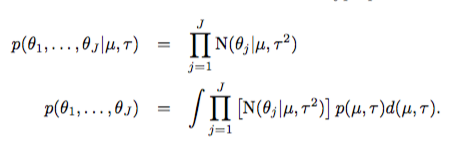
\includegraphics[scale = 0.5]{spec1.png}
\end{center}
i.e. the $\theta_j$ are conditionally independent given $(\mu, \tau)$ We also assign a non informative uniform hyperprior distribution to $\mu$, given $\tau$.
\begin{center}
    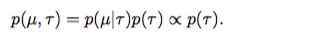
\includegraphics[scale = 0.52]{spec2.png}
\end{center}

Our joint posterior can be expressed in terms of the sufficient statistics

\begin{center}
    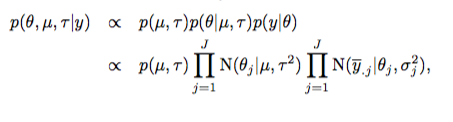
\includegraphics[scale = 0.5]{spec3.png}
\end{center}

The conditional posterior distributions for for $\theta_j$ becomes 
\begin{center}
     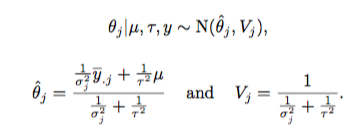
\includegraphics[scale = 0.5]{spec4.png}
\end{center}

The remaining specifications are listed below
\begin{center}
    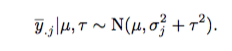
\includegraphics[scale = 0.55]{spec5.png}\\
    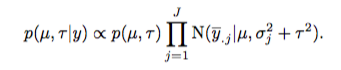
\includegraphics[scale = 0.55]{spec6.png}\\
    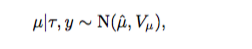
\includegraphics[scale = 0.55]{spec7.png}\\
    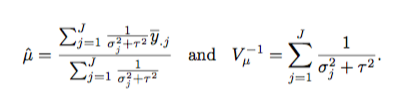
\includegraphics[scale = 0.55]{spec8.png}\\
    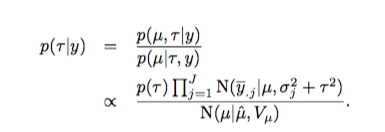
\includegraphics[scale = 0.55]{spec9.png}\\
    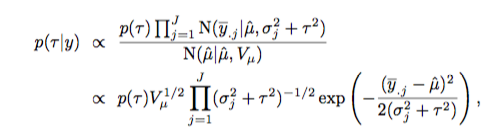
\includegraphics[scale = 0.55]{spec10.png}\\
    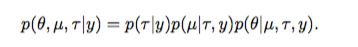
\includegraphics[scale = 0.55]{spec11.png}
\end{center}

\section{Direct Sampling}
In simple non-hierarchical Bayesian models, it is often easy to draw from the posterior distribution directly, especially if conjugate prior distributions have been assumed. Frequently, draws from standard distributions or low-dimensional non-standard distributions are required, either as direct draws from the posterior distribution of the estimand in an easy problem, or as an intermediate step in a more complex problem.

\subsection{Procedure}
For the simplest discrete approximation, compute the target density, $p(\theta|y)$, at a set of evenly spaced values $\theta_1,...,\theta_N$ that cover a broad range of the parameter space for $\theta$, then approximate the continuous $p(\theta|y)$ by the discrete density at $\theta_1,..., \theta_N$ , with probabilities ${p(\theta_i|y)}/{\suml p(\theta_l|y)} $. Because the approximate density must be normalized anyway, this method will work just as well using an unnormalized density function, $q(\theta|y)$, in place of $p(\theta|y)$.


Once the grid of density values is computed, a random draw from $p(\theta|y)$ is obtained by drawing a random sample Uniform distribution on [0, 1], then transforming by the inverse cdf method to obtain a sample from the discrete approximation. When the points $\theta_i$ are spaced closely enough and miss nothing important beyond their boundaries, this method works well. 


% Once we have a sample from the posterior distribution, $p(\theta|y)$, we draw from the predictive distribution of unobserved or future data, $\Tilde{y}$. For each draw of $\theta$ from the posterior distribution, just draw one $\Tilde{y}$ from the predictive distribution, $p(\tilde{y}|\theta)$. The set of simulated $\tilde{y}$'s from all the $\theta$ characterizes the posterior predictive distribution. 

\section{Results}
\begin{figure}[h!]
    \centering
    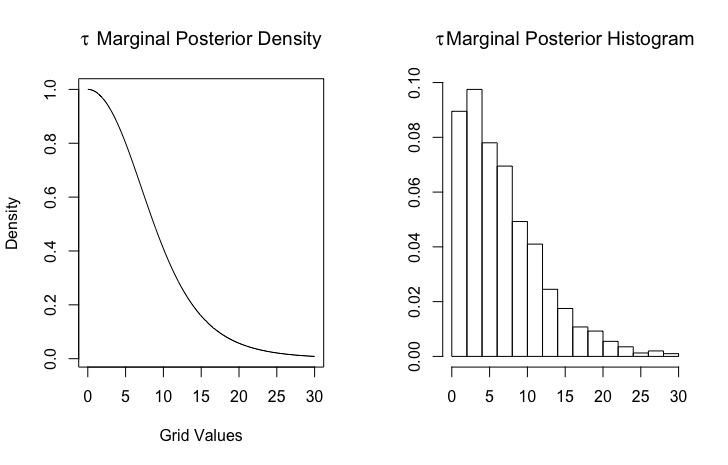
\includegraphics[scale =0.6]{DS_Tau.png}
    \caption{Direct Sampling: Marginal posterior density and histogram, $p(\tau|y)$, for standard deviation of the population of school effects $\theta_j$ in the educational testing example.
}
    \label{DS_tau}
\end{figure}

\begin{figure}[h!]
    \centering
    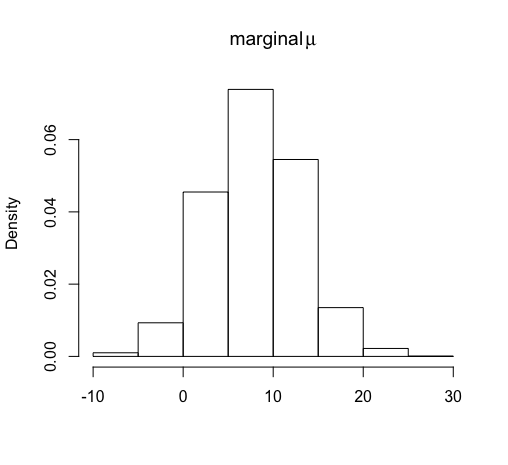
\includegraphics[scale = 0.4]{DS_mu.png}
    \caption{Marginal posterior histogram for $\mu$.}
    \label{DSMu}
\end{figure}

\begin{table}[h!]
\centering
\label{DSTheta}
\caption{The Direct Sampling Summary of 2000 simulations of the treatment effects in the eight schools.}
\begin{tabular}{rrrrr}
  \hline
$\theta_j $ & mean & sd & 0.025 & 0.975 \\ 
  \hline
1 & 12.37 & 8.58 & -1.62 & 33.21 \\ 
  2 & 8.27 & 6.54 & -4.45 & 21.08 \\ 
  3 & 6.75 & 8.12 & -10.49 & 22.13 \\ 
  4 & 7.98 & 6.75 & -5.18 & 21.64 \\ 
  5 & 5.81 & 6.50 & -7.80 & 17.60 \\ 
  6 & 6.36 & 6.98 & -8.50 & 18.91 \\ 
  7 & 10.98 & 6.87 & -1.26 & 26.19 \\ 
  8 & 8.74 & 8.27 & -7.48 & 25.94 \\ 
   \hline
\end{tabular}
\end{table}

\begin{figure}[h!]
    \centering
    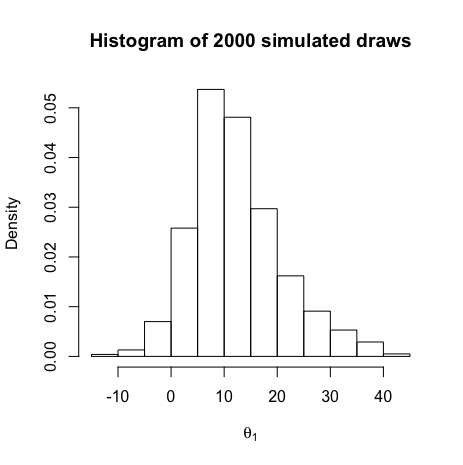
\includegraphics[scale = 0.4]{DStheta1.png}
    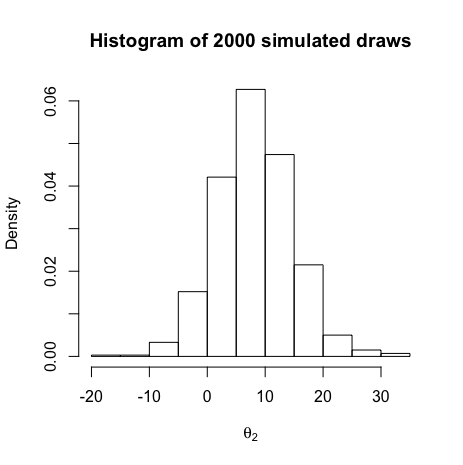
\includegraphics[scale = 0.4]{DStheta2.png}
    \caption{Histograms of two quantities of interest computed from the 2000 simulatied draws of the effect in school A, $\theta_1$, and the effect in school B, $\theta_2$.}
    \label{fig:my_label}
\end{figure}

\begin{figure}[h!]
    \centering
    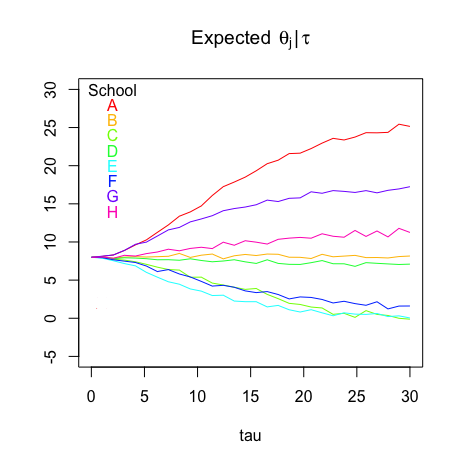
\includegraphics[scale = 0.5]{DSSchool.png}
    \caption{Conditional posterior means of treatment effects, $E(\theta_j |\tau, y)$, as functions of the between  school standard deviation $\tau$, for the educational testing example. The line for school C crosses the lines for E and F because C has a higher measurement error ) and its estimate is therefore shrunk more strongly toward the overall mean in the Bayesian analysis.}
    \label{LinesDS}
\end{figure}
\clearpage
\section{Gibbs Sampling}
Here we wish to draw random samples from the joint posterior given by
\begin{center}
    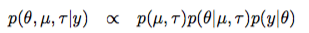
\includegraphics[scale =0.55]{jointPost.png}
\end{center}
On the right hand side of the proportionality statement we have defined each of these in closed form, thus a Gibbs sampling algorithm is appropriate. 
\begin{table}[ht]
\centering
\label{gibbstab}
\caption{The Gibbs Sampling Summary of 2000 simulations of the treatment effects in the eight schools. There is clearly a slight difference in certain values for the posterior expected mean for $\theta$, but it is clearly comparable to Direct sampling}

\begin{tabular}{rrrrr}
  \hline
parameter & Mean & SD & 0.025\% & 0.975\% \\ 
  \hline
$\theta_1$ & 14.97 & 10.40 & -2.20 & 39.04 \\ 
  $\theta_2$ & 8.04 & 7.52 & -7.10 & 23.72 \\ 
  $\theta_3$ & 4.76 & 9.91 & -16.78 & 23.74 \\ 
  $\theta_4$ & 7.64 & 7.81 & -8.43 & 23.09 \\ 
  $\theta_5$ & 3.49 & 7.35 & -12.13 & 17.41 \\ 
  $\theta_6$ & 4.77 & 8.18 & -12.45 & 20.03 \\ 
  $\theta_7$ & 12.56 & 8.17 & -1.94 & 30.05 \\ 
  $\theta_8$ & 9.22 & 10.40 & -11.27 & 30.39 \\
  $\mu$ & 8.07 & 6.67 & -4.81 & 21.07 \\ 
  $\tau$ & 12.06 & 8.98 & 1.81 & 33.24 \\ 
   \hline
\end{tabular}
\end{table}
\begin{center}
    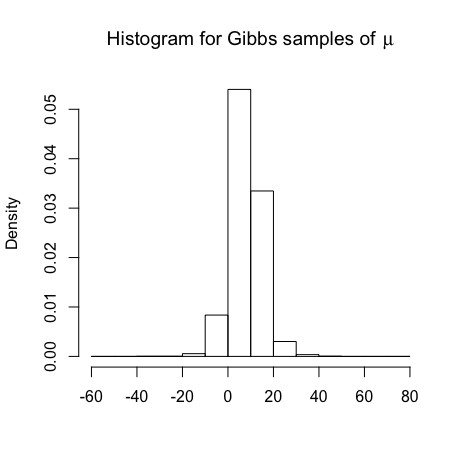
\includegraphics[scale = 0.5]{gibbs_mu.png}
    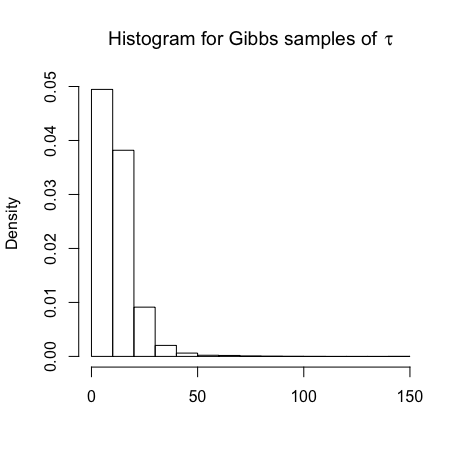
\includegraphics[scale = 0.5]{gibbs_tau.png}
\end{center}

Most of what is seen above appears different than the direct sampling method. So we examine the trace plots and auto correlation plots to see if mixing is occuring properly.

(ADD PLOTS)
\section{Abrams \& Sans\`o}
From [Abrams \& San\`so 1998] we define the following model specifications:
\begin{align*}
    y_i \sim& N(\theta_i, \sigma_i^2/n)\\
    \theta_i \sim& N(\mu, \tau^2)\\
    \sigma_i^2 \propto& 1/\sigma_i^2\\
    \tau^2 \sim& IG(a,b)\\
    \mu \sim& Unif(0,1)
\end{align*}
According to the paper, the prior on $\sigma_i^2$, chosen to be Jeffrey's prior is due to the fact that in practice little information is likely to be available about the within-study variances. A prior distribution for $\tau^2$ has to be flexible enough to be able to easily accommodate a priori
information whilst at the same time being mathematically convenient. For this reason, the paper suggests placing an inverse
gamma distribution with parameters a and b. A vague Uniform prior is suggested to be placed on $\mu$.

we have an approximation for the first moment of the effect of the ith school as described in the SAT model is given by
\begin{align*}
    E(\theta_i|y, s^2, n) \approx y_i - \frac{(n_i - 1) s_i^2 b (2a + k - 1}{2 n_i (n_i -3) (1 +bRSS_B/2}(y_i - \overline{y})
\end{align*}
where $RSS_b = \sum_i y_i^2 - k\overline{y}^2$, the residual sum of squares between studies (schools) and $a$ and $b$ are the hyper parameters of the inverse gamma prior on $\tau$. We also have the following approximations
\begin{center}
    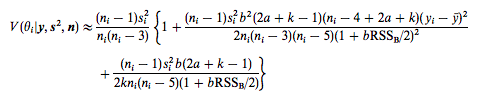
\includegraphics[scale = 0.7]{paper1.png}\\
    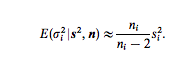
\includegraphics[scale = 0.7]{paper2.png}\\
    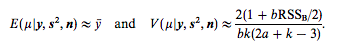
\includegraphics[scale = 0.7]{paper3.png}\\
    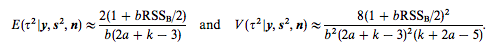
\includegraphics[scale = 0.7]{paper4.png}\\
    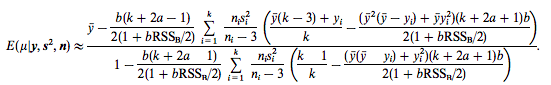
\includegraphics[scale = 0.7]{paper5.png}
\end{center}

These are written as in the paper, but I was not getting sensible results at first until. I was using very odd choices for the parameters of the Inverse gamma prior on $\tau^2$. Using $a=2$ and $b = 50$, I obtained the following (I will be asking you about this later because Some of these seem close, but the theta's are not so I am curious if there is also a typo in the paper? for this reason I exclude the approximations for thetas.)
\begin{center}
\begin{tabular}{ll}
\hline
\hline
     $E(\mu|y,s^2,n) \approx 8.5$ & $V(\mu|y,s^2,n) \approx 79.98$  \\
     $E(\tau|y,s^2,n) \approx 18.03$ & $V(\tau|y,s,n) \approx 116.179$\\
     \hline\hline
\end{tabular}
\end{center}
\section{Conclusion}
I wanted to write a better conclusion and interpret the results better, but I did not manage my time well. Please enjoy this meme that I will probably attach to every homework because it never gets old! 
\begin{figure}[b!]
    \centering
    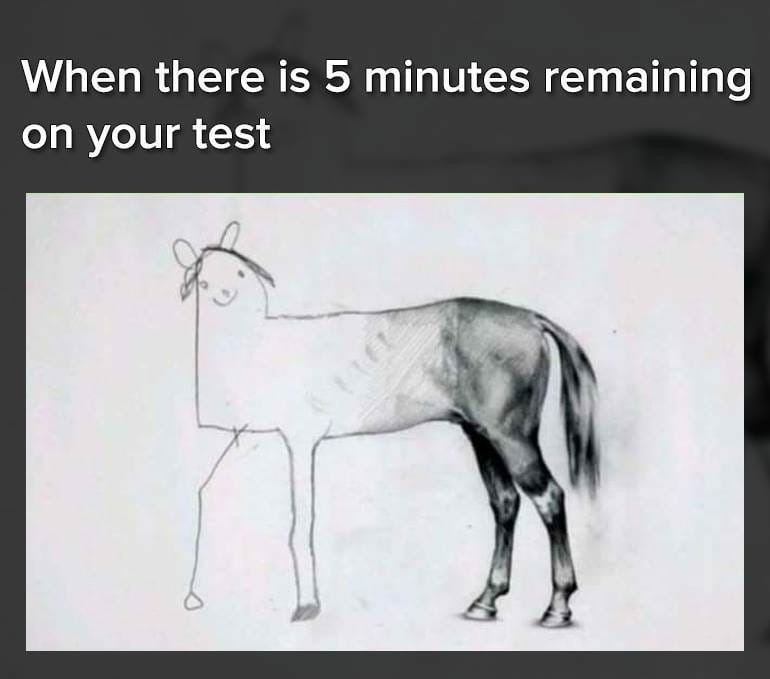
\includegraphics[scale=0.2]{IMG.JPG}
\end{figure}

\end{document}
